\chapter{Implementierung}\label{ch:Implementierung}

Dieses Kapitel wird sich der Implementierung der Thesis widmen. Es wird gezeigt, wie die Konzeption als Software umgesetzt wurde und einige wichtige Code-Stücke vorgestellt. Die Implementierung wurde auf dem \ac{ROS}-Framework aufgebaut.

\section{Generelles zur Implementierung}
Die Implementierung baut auf Ubuntu LTS 16.04 mit der \ac{ROS}-Version 'Lunar' auf, da diese beiden Komponenten das derzeit stabilste Duo bilden. Aufgrund mangelnder Kapazitäten, befindet sich das Ubuntu-System in einer Virtuellen Maschine, was, bis auf einen höheren Ressourcen-Verbrauch, allerdings keinerlei erkennbare Nachteile mit sich zog.

Generell ist das \ac{ROS}-Framework in C++ und Python verfügbar, wobei diese Sprachen gemischt werden könnten, wenn sie auf verschiedenen Nodes genutzt werden. Als Programmiersprache wurde letztlich C++ verwendet, da es deutlich besser mit den verfügbaren Ressourcen umgeht. In den späteren Auswertungen hat sich diese Wahl positiv bestätigt, da 25 gleichzeitige Roboter eine Menge Ressourcen verschlungen haben und den verfügbaren Computer (auch wegen der VM) bereits an die Grenzen seiner Leistung brachte.

Da ein experimentelles Vorgehen direkt an realen Robotern zu Aufwändig wäre, insbesondere was die Zeitkosten für die Durchführung und Auswertung einer Simulation angeht, beruht die Implementierung auf der Node Turtlesim\cite{ROS_TURTLESIM} von ROS~(siehe~\autoref{subsec:Grundlagen_Turtlesim}). Die Turtlesim wurde dahingehend angepasst, dass die Bilder der Turtles durch wesentlich kleinere Bilder schwarzer Pfeile ersetzt wurden die visuellen Aufschluss auf Position und Aurichtung erlauben. Dadurch wurde mehr Platz und Übersichtlichkeit gescahffen. Das Verhalten der Turtles selbst in der Simulation ist unverändert.

Grundsätzlich ist die Turtlesim nicht dafür gemacht worden um aufwändigere Simulationen zu erproben. Der Zweck ist es einen einfachen Einstieg in das \ac{ROS}-Framework zu geben und Neulinge durch die Tutorials zu begleiten. Sie bietet aber eine grafische Oberfläche, die bei der Implementierung sehr nützlich ist, insbesondere um Fehler besser entdecken zu können.
Bei der Implementierung wurde viel Wert auf eine modulare Bauweise gesetzt. Die Bewegungsbefehle die aktuell an die Turtlesim gehen sind abstrahiert und lassen sich später schnell auf das System des jeweiligen Roboters umschreiben. Andere Nachrichten gehen nicht über die Turtlesim, wodurch die Bewegung das einzige Sub-System ist, dass es nachher anzupassen gilt.

\section{Nachbau des Schwarms nach Craig Reynolds}

Sendet man einen Bewegungs-Befehl an die Turtlesim, wird diese den Befehl für 1 Sekunde ausführen und nach Abschluss die Position des Roboters automatisch an die Subscriber verteilen. Die Subscriber erhalten in \ac{ROS} ihre Informationen immer über Callback-Funktionen. Da diese Funktionen statisch sein müssen, ist es nicht einfach möglich die Daten in einem Objekt zu speichern, sondern sie müssen in globalen Variablen untergebracht werden.
Die Informationen über die Position der Roboter werden in einem Array gespeichert. Da die Roboter IDs haben, ist es leicht diese bei 0 beginnen zu lassen und sie dann als Index zur Adressierung innerhalb des Arrays zu nutzen.

\begin{wrapfigure}{r}{\pictureWidthBig}
	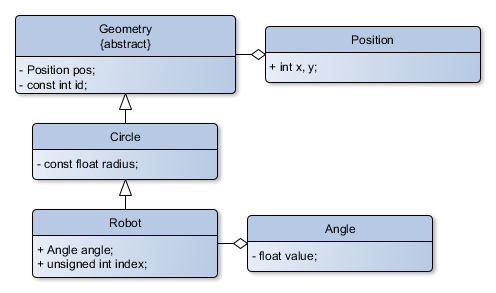
\includegraphics[width=\pictureWidthBig,keepaspectratio]{graphics/Klassendiagramme/KlassendiagrammRobot.png}
	\caption{Die Klassenhierarchie eines Roboter-Objektes}
	\label{pic:KlassendiagramRoboter}
\end{wrapfigure}

Da Roboter eine Position und eine Fläche haben die deren Körper darstellt, macht es am meisten Sinn ihnen einen Kreis als geometrische Form zu vererben, sodass letztlich die Klassen-Struktur aus \autoref{pic:KlassendiagramRoboter} entsteht (Funktionen wurden ausgelassen). Der Nutzen der Klasse \highlight{Angle} ist der, dass die Klasse automatisch darauf achtet im Bereich [0, 360] zu bleiben: \highlight{Angle(350) + Angle(20) == Angle(10)}.

\subsection*{Messages}

Die Steuerung der Roboter innerhalb der Turtlesim geschieht nicht direkt durch das eigene Programm. Stattdessen müssen Nachrichten an die Turtlesim gesendet werden die dann letztlich die Roboter bewegt. Insgesamt werden dafür 5 Nachrichten verwendet. Die Nachrichten-Typen werden der Übersichtlichkeit halber in einer verkürzten Schreibweise vorgestellt, wie sie in \ac{ROS} nicht erlaubt, von Programmiersprachen wie C++ oder Java, aber bekannt ist. Einige Nachrichten arbeiten mit dem Topic 'turtleX', was nichts anderes bedeutet als eine ID für die Roboter der Turtlesim (turtle1, turtle2, ...).

\begin{lstlisting}[style=ros, title=turtlesim/Pose.msg]
	// Empfangen von dem Topic: turtleX/pose
	// Gibt Feedback zur Position und Ausrichtung des Roboters
	// Wird in dieser Arbeit genutzt, um die Position der Roboter zu speichern
	float32 x, y, theta, linear_velocity, angular_velocity
\end{lstlisting}

\begin{lstlisting}[style=ros, title=geometry\_msgs/Twist.msg]
	// Gesendet an das Topic: turtleX/cmd_vel
	// Fahrbefehl fuer den Roboter, wird 1 Sekunde lang ausgefuehrt
	// Wird in dieser Arbeit genutzt, um die Roboer geradeaus zu fahren zu lassen
	Vector3  linear, angular
\end{lstlisting}

\begin{lstlisting}[style=ros, title=turtlesim/TeleportRelative Service]
	// Gesendet an den Service: turtleX/teleport_relative
	// Teleportiert den Roboter zu einem relativen Ort
	// Wird in dieser Arbeit genutzt, um die Roboter vor dem Fahrbefehl zu drehen
	float32 linear, angular
	---
\end{lstlisting}


\newpage
\begin{lstlisting}[style=ros, title=turtlesim/Spawn Service]
	// Gesendet an den Service: spawn
	// Erschafft einen neuen Roboter in der Turtlesim
	float32 x, y, theta
	string name
	---
	string name
\end{lstlisting}

\begin{lstlisting}[style=ros, title=turtlesim/SetPen Service]
	// Gesendet an den Service: turtleX/set_pen
	// Schaltet den Pen aus. Ein 'Stift' der den gefahrenen Weg markiert
	uint8 r, g, b, width, off
	---
\end{lstlisting}

\subsection*{Unterscheiden der einzelnen Pose-Callbacks}

Die Turtlesim verbreitet die Position der Roboter nach jedem Bewegungsbefehl. Leider ist in der Nachricht \highlight{Pose.msg} keinerlei Information darüber enthalten, von wem die Nachricht kommt.

\begin{lstlisting}[style=cpp, title=Callback-Funktion für Pose.msg]
void flockCallback(const turtlesim::PoseConstPtr &msg);
\end{lstlisting}

Um die Nachrichten nun den einzelnen Robotern zuordnen zu können, gäbe es nun die Möglichkeit jedem Callback eine eigene Callback-Funktion zuzuordnen. Diese Methode wäre allerdings Handarbeit und nicht dynamisch. Braucht man mehr (oder weniger) Roboter, müsste man die Funktionen eigenhändig umändern.
Einen kleinen Trick um dies nicht tun zu müssen, bietet die Boost-Bibliothek mit der \ac{ROS} arbeitet. Mit Hilfe dieser kann man einer Methode einen weiteren, festen Parameter zuordnen.

\begin{lstlisting}[style=cpp, title=Callback-Funktion für Pose.msg mit Boost]
void flockCallback(const turtlesim::PoseConstPtr &msg, const unsigned int index);

std::vector<ros::Subscriber> flockSubscriber;
void subscribeToFlock() {
    ros::NodeHandle node;

    for (int i = 0; i < FLOCK_SIZE; i++) {
        boost::function<void(const turtlesim::PoseConstPtr &)> callback = bind(flockCallback, _1, i);
        flockSubscriber.push_back(node.subscribe("turtle" + std::to_string(i) + "/pose", 100, callback));
    }
}
\end{lstlisting}

Dadurch lassen sich alle Callbacks auf die selbe statische Methode verlinken, bei Aufruf wird jedoch immer ein zusätzlicher, fester Parameter mit eingebunden. Die Callbacks können nun in einer Schleife abgearbeitet werden und die Dauer der Schleife als konstanter Parameter codiert werden.
Eine ähnliche (wenn nicht sogar die selbe) Klasse hat es mit dem Standard C++11 auch in den STL-Header \highlight{<functional>} geschafft\cite{CPP_REFERENCE_FUNCTION}. Da \ac{ROS} aber intern mit der Version von Boost arbeitet\cite{BOOST_REFERENCE_FUNCTION}\cite{ROS_SOURCE_NodeHandle}, ist man dazu gezwungen deren Version zu nutzen und nicht die der STL.

\subsection*{System-Takt: Ticks}\label{subsec:Tick}

Der Ablauf eines Programms geschieht in Ticks (der Takt des Systems, periodische Zeitabstände), in denen zuerst eine Aktion gestartet und danach eine kurze Zeit gewartet wird um Nachrichten anderer Roboter zu empfangen und zu verarbeiten. Es ist damit implizit nur eine Bewegungs-Aktion pro Tick möglich. Diese kann allerdings Drehung und Fahren kombinieren.
Die Bewegung eines Roboter wird von \ac{ROS} genau 1 Sekunde lang ausgeführt\footnote{\url{http://wiki.ros.org/turtlesim\#Subscribed_Topics}}. Die Steuerung der bewegten Entfernung pro Tick lässt sich daher nur über die Geschwindigkeit der Bewegung steuern. In der Praxis hat sich aufgrund von weiteren Verzögerungen in der Turtlesim eine Tick-Länge von 1.1 Sekunden bewährt um sicherzustellen, dass die \highlight{Pose.msg} der Turtlesim auch rechtzeitig ankommt. \ac{ROS} bietet dafür eine bequeme Funktion mit seiner Klasse \highlight{ros::Rate} und deren Funktion \highlight{sleep()}.

\begin{lstlisting}[style=cpp, title=Ticks abschließen mit ROS Funktionen]
ros::Rate sleeper(0.9);
        
while (true) {
	// do something
	sleeper.sleep();
	ros::spinOnce();
}
\end{lstlisting}

Der Konstruktor nimmt einen float entgegen der die Frequenz angibt. Die wirkliche Länge der Ticks beträgt also 1.111 Sekunden. Der Funktionsaufruf \highlight{sleeper.sleep()} blockiert solange, bis der letzte Aufruf (innerhalb des gleichen Objektes) 1.111 Sekunden her ist. Braucht das Programm zwischen den Aufrufen länger als die Periode lang ist, kehrt die Funktion entsprechend sofort zurück.
Während der Wartezeit gehen (hoffentlich) alle neuen Positionsdaten der anderen Roboter ein. Nach der Wartezeit werden diese dann abgearbeitet und das Programm arbeitet an seinem nächsten Zyklus.

Entschließt sich ein Roboter dazu sich nicht zu bewegen, muss er einen 'leeren' Bewegungsbefehl senden, der dazu führt, dass sich der Roboter nicht bewegt und somit einen Tick abschließen, statt einfach zu warten und nichts zu senden. Der Grund hierführ liegt darin, dass die Systeme Single-Thread Architekturen sind und das Abfragen der Topics explizit ausgelöst werden muss. Dies geschieht über die Funktion \highlight{ros::spinOnce()} von \ac{ROS}. Diese Funktion bewirkt, dass \ac{ROS} alle Callback-Funktionen der entsprechenden eingegangenen Events aufgerufen werden. Es werden also die bisher eingegangenen\highlight{Pose.msg}s durch ihre Callbacks verarbeitet. Außerdem werden dadurch die eigenen Daten auf den Robotern aufgefrischt und eventuelle Informationen gesendet, die nichts mit der Bewegung zu tun haben. Das Abschließen eines Ticks synchronisiert somit generell die Daten des eigenen Systems mit dem der anderen.

Die Ticks sind trotz allem keine globalen Ticks, die jeden Roboter gleichzeitig betreffen. Jeder Roboter arbeitet auf seiner 'Zeitlinie' und agiert unabhängig der Ticks der anderen Einheiten.

\subsection*{Einhalten der 4 Grundregeln}
Die Roboter wurden als autonome Einheiten konzipiert die sich ausschließlich anhand von 3 fixen Parametern bewegen und dabei versuchen die 4 Grundlegen des Schwarmverhalten einzuhalten. Grundsätzlich werden von einem Roboter nur andere Einheiten beachtet, die in einem gewissen Radius um ihn herum positioniert sind. Daher wird Am Anfang eine Liste derjenigen erstellt. Dies geschieht durch simples iterieren über die Liste aller Roboter und einer Berechnung über Pythagoras.

\subsubsection*{Ausrichtung: Passe deine Bewegungsrichtung deinen Nachbarn an}

\begin{wrapfigure}{r}{\pictureWidthSmall}
	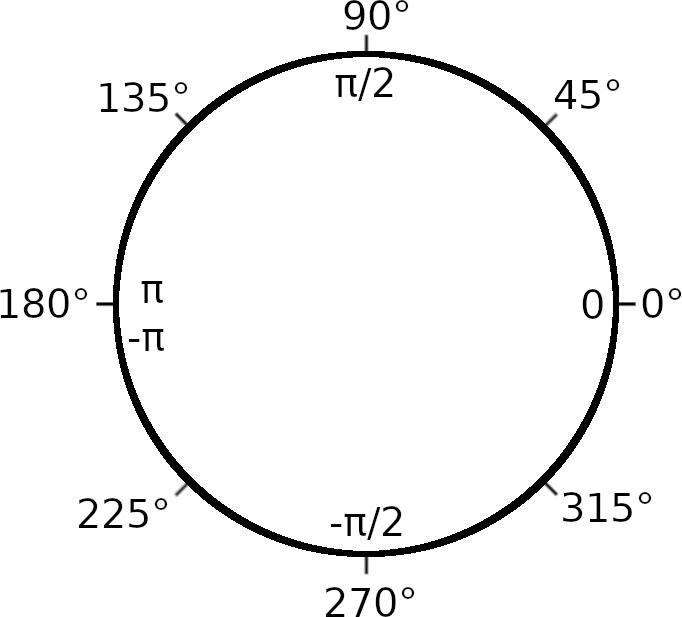
\includegraphics[width=\pictureWidthSmall,keepaspectratio]{graphics/WinkelTemplate.png}
	\caption{Winkel-Übersicht}
	\label{pic:WinkelUebersicht}
\end{wrapfigure}

Die Turtlesim selbst arbeitet bei Winkeln mit dem Bereich von [-3.14, 3.14], wohingegen die Steuerung der Roboter mit dem Bereich [0°, 360°] arbeitet, da dieser besser bearbeitet (und von Menschen gelesen) werden kann. Außerdem ist dadurch generell eine Abstraktions-Ebene entstanden, die es später erlaubt mit jedem bliebigen anderen Winkel-System zu arbeiten.
Eintreffende Positionsdaten, von anderen Robotern, müssen also erst in die interne Darstellung umgerechnet werden. Ebenso wird der Winkel vor dem Senden eines Bewegungs-Befehls automatisch so umgerechnet, dass die Turtlesim ihn akzeptiert. Wird der Turtlesim ein zu großer Winkel gesendet, z.B.: 5, so wird der überschüssige Winkel einfach abgezogen und es wäre eine Drehung um 1.86. In~\autoref{pic:WinkelUebersicht} ist eine Übersicht über die Winkel zu sehen wie sie im System und von der Turtlesim genutzt werden.

\begin{lstlisting}[style=cpp, title=Berechnung der mittleren Ausrichtung eines Schwarms]
Angle meanAngle(const std::vector<Angle> &angles) {
    double y_part = 0, x_part = 0;

    for (const Angle &angle : angles) {
        x_part += std::cos(angle.get() * M_PI / 180.0f);
        y_part += std::sin(angle.get() * M_PI / 180.0f);
    }

    return Angle(x_part / angles.size(), y_part / angles.size());
}

Angle::Angle(float vec_x, float vec_y) {
    this->value = std::atan2(vec_y, vec_x) * 180.0f / M_PI;
    normalize(); // value = value % 360.0f;
}
\end{lstlisting}

 
\subsubsection*{Zusammenhang: Versuche deinen Nachbarn nahe zu sein}

Für die Berechnung des Mittelpunkts der Nachbarschaft, wurde schlicht die Liste der Roboter, die nahe genug sind, genommen und ein mathematischer Durchschnitt gebildet. Die Koordinaten wurden danach von den eigenen abgezogen und die resultierenden X/Y-Werte als Vektoren genutzt um den Winkel zu berechnen, den der Mittelpunkt zum Roboter hat. Anschließend wurde die Differenz dieses Winkels zu dem eigenen Winkel gebildet, den man vorher fahren wollte.
Von diesem entstandenen Winkel wird nun ein prozentualer Wert genommen (je nach Einstellung des Parameters) und vom ursprünglichen Winkel abegzogen.

\begin{lstlisting}[style=cpp, title=Berechnung des Fahrtwinkels]
Angle RobotPilot::nextStep() {
	const std::vector<Robot> &flock = findFlock(self());
	Angle turnAngle = averageDegree(flock);
	addFreeWill(turnAngle);

	const Angle &angleToFlockCentre = self().angleTo(flockCentre(flock));
	turnAngle += (angleToFlockCentre - turnAngle) * FLOCK_TURN_TO_FLOCK_PERCENT;

	return turnAngle;
}
\end{lstlisting}

\subsubsection*{Abschottung: Vermeide Kollisionen mit deinen Nachbarn}

Um Kollisionen mit anderen Robotern zu vermeiden, werden zur Kollisionserkennung interne Simulationen verwendet. Im Grunde bedeutet dies, dass berechnet wird wo der Roboter mit dem aktuell gewünschten Winkel und normaler Geschwindigkeit hinfahren wird. Ist dieser Ort weit genug von anderen Robotern entfernt, wird er akzeptiert. Ist er es nicht, wird der gewünschte Winkel in Schritten von 1° erst nach links und dann nach rechts verändert und erneut geschaut ob es am Zielort zu einer Kollision kommen wird.

\begin{lstlisting}[style=cpp, title=Simulation auf Kollisionen am Zielpunkt]
bool RobotPilot::predictRobotCollision(const Position &destination) const {
        for (const Robot &robot : globalSwarm) {
            if ((robot != self()) and robot.inBoundary(destination)) {
                return true;
            }
        }

        return false;
}
\end{lstlisting}

\paragraph*{Unzureichende Erkennung auf dem Weg}
Um die Berechnung einfacher zu gestalten und Ressourcen zu schonen wurde nicht der Weg selbst überprüft. Es ist also möglich, dass ein Roboter weder auf seinem Ursprungs- oder Zielort mit anderen Robotern kollidiert, wohl aber auf dem Weg dorthin. Ebenfalls ist es in der Turtlesim nicht möglich, eine angefangene Bewegung wieder abzubrechen. Kommt es also während der Ausführung zu einer Kollision, z.B. weil sich zwei Roboter aufeinander zubewegen, kann diese nicht mehr verhindert werden. Ein Ausgleich in der Simulation ist durch eine Abfrage gegeben, ob sich zwei Roboter 'ineinander' befinden. Die entsprechenden Roboter werden dann auf direkter Luftlinie voneinander weggeschoben, um wieder einen plausiblen physikalischen Zustand einzunehmen.

Im der Praxis sollte eine Kollision auf dem Weg kein Problem darstellen, da mit parallelen Threads nebenläufiges Verhalten eingesetzt werden kann. Außerdem ließe sich, im Falle einer Single-Thread-Architektur, die Frequenz der Ticks wesentlich schneller eingestellen, sodass sich die Roboter effektiv nur wenige Millimeter pro Tick bewegen, dafür aber mit über 100 Ticks pro Sekunde.% Letztlich kommt es auf die Leistung des verwendeten Computers an.

\subsubsection*{Flucht: Fliehe vor Dingen, die eine potentielle Gefahr darstellen}

\begin{wrapfigure}{r}{\pictureWidthBig}
	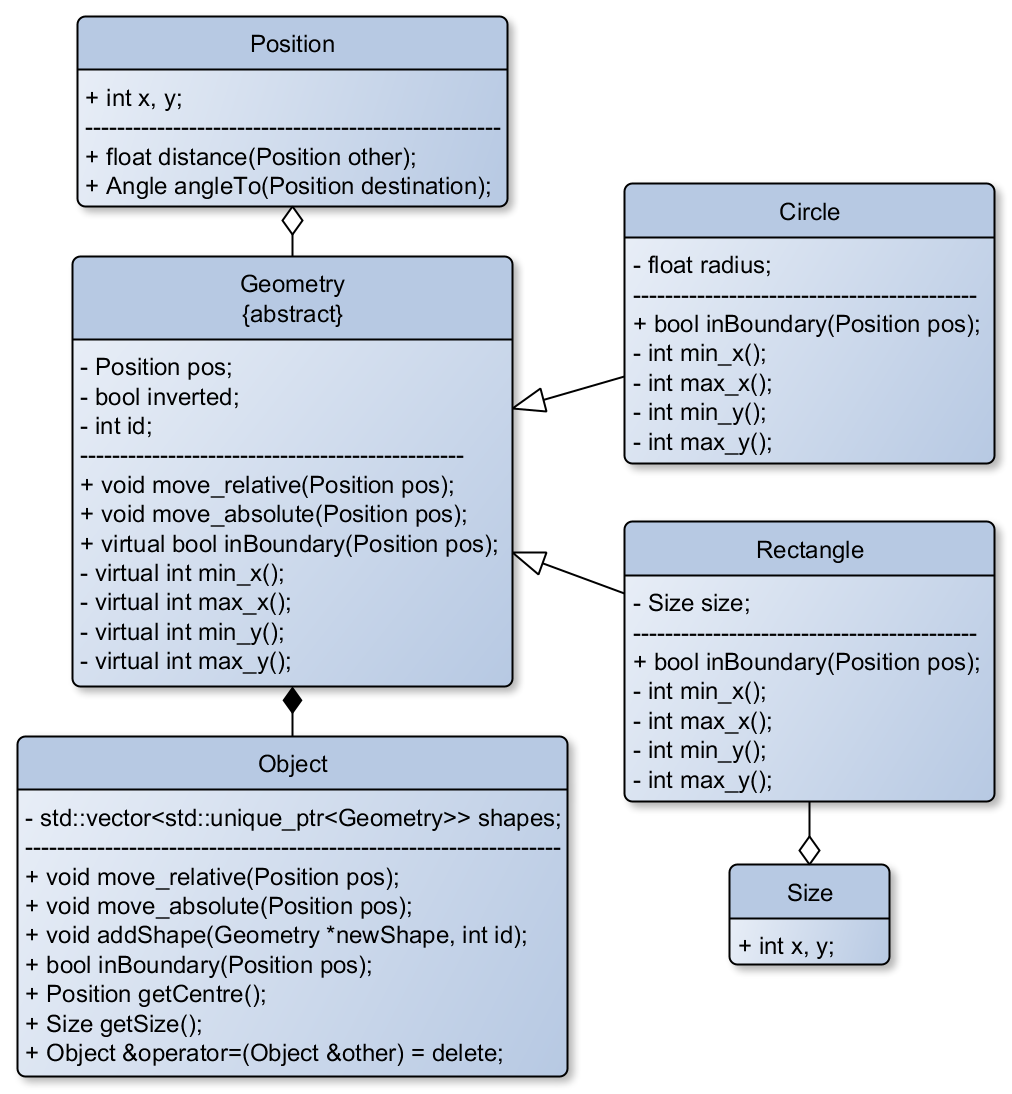
\includegraphics[width=\pictureWidthBig,keepaspectratio]{graphics/Klassendiagramme/KlassendiagrammObject.png}
	\caption{Die Klassenhierarchie eines Hindernisses}
	\label{pic:KlassendiagramObjekt}
\end{wrapfigure}

Kollisionen mit Gefahrenzonen werden erkannt, indem über ein globales Array von \highlight{Object}-Klassen iteriert wird und die einzelnen Objekte nach Kollisionen auf den genannten Koordinaten gefragt werden. Es muss nur die \highlight{Object}-Klasse nach einer Kollision befragt werden, diese leitet die Anfrage an alle Geometrien weiter. Wird eine Kollision bei einem Objekt erkannt, wird sie genau wie bei der Kollision mit Robotern durch iterativ steigendes Ausweichen zu beiden Seiten verhindert.
Um Gefahrenzonen darzustellen, wird auf Abstraktion und Vererbung gesetzt. Es gibt, wie in \autoref{pic:KlassendiagramObjekt} zu sehen ist, eine Hierarchie von Klassen aus denen sich die Zonen zusammensetzen lassen. Die \highlight{Geometry}-Klassen die sich in der \highlight{Object}-Klasse befinden, werden alle von dieser gesteuert. Bewegt sich das Objekt, bewegen sich alle darin enthaltenen Geometrien. Das Hinderniss bleibt dadurch immer in einem plausiblen Zustand. 


%\subsection*{Berechnung der Bewegung}
%
%Die Berechnung der Bewegung geschieht letztlich in den Schritten die in \autoref{pic:AblaufSchwarm} gezeigt werden.

%\begin{wrapfigure}{r}{\pictureWidth}
%	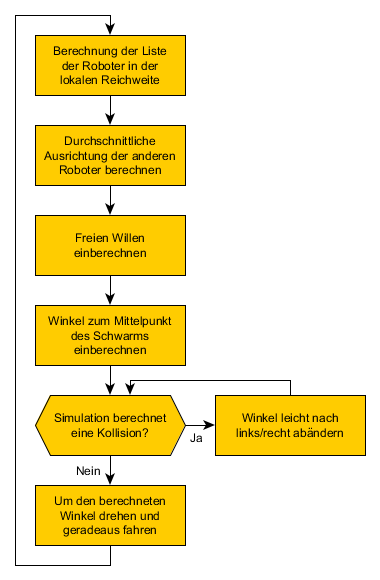
\includegraphics[width=\pictureWidth,keepaspectratio]{graphics/ImplSchwarm.png}
%	\caption{Ablaufdiagramm Schwarm}
%	\label{pic:AblaufSchwarm}
%\end{wrapfigure}









\section{Anführer}

Da der Anführer seinen Schwarm lenkt, verfällt die Einheit, die zum Anführer wurde, in ein spezielles Verhalten. Dieses Verhalten ist ein neuer Zweig im Programm der Roboter, welches von dem Verhalten des normalen Schwarmroboter gänzlich abweicht. Auf das Ziel zuzusteuern und den Schwarm dabei nicht zu verlieren, ihn sogar wieder einzufangen, wenn er abhanden kommt, kann mit den bisherigen Schwarmregeln nicht umgesetzt werden. Aus diesem Grund ist die Implementierung weniger ein umändern der bisherigen Implementierung, sondern es wird eher ein neues Verhalten hinzugefügt und eine Abzweigung im Code um dieses auszuführen.

Generell ist der Anführer frei von den Verhaltensweisen des sonstigen Schwarms. Weder verfügt er über einen freien Willen, noch versucht er seinem Schwarm nahe zu sein, in dem Sinne in dem es bisher Implementiert wurde. Auch die Orientierung an der Ausrichtung anderer Roboter entfällt vollständig, da er sich auf sein Ziel ausrichten muss.

\newpage\subsection*{Generelles Verhalten}

\begin{wrapfigure}{r}{\pictureWidthBig}
	\includegraphics[width=\pictureWidthBig,keepaspectratio]{graphics/ImplAnführer.png}
	\caption{Ablaufdiagramm Schwarm}
	\label{pic:AblaufAnführer}
\end{wrapfigure}

\autoref{pic:AblaufAnführer} zeigt das Verhalten wie es umgesetzt wurde.
Der Anführer ist ein Zweig im normalen Verhalten der Roboter. Erhält ein Roboter eine Nachricht vom Typ \highlight{New\_Mission} und seine ID entpricht der ID in der Nachricht, richtet er sich nach diesem Ziel aus und fährt ihm entgegen. Behindert ein anderer Roboter, dass der Anführer geradeaus weiter kann, verringert er seine Geschwindigkeit oder bleibt letztlich einen Tick lang stehen. Ist er nahe genug am Ziel angekommen, fällt er in sein altes Verhalten zurück. \autoref{pic:AblaufAnführer} zeigt das implementierte Verhalten des Anführers.

Das Einfangen des Schwarms, wenn dieser sich zu weit entfernt, ist widerum eine Subroutine im Verhalten des Anführers. Ist diese Routine gestartet, bleibt er in diesem Zustand, bis sie vollständig ausgeführt ist und der Schwarm wieder eingefangen wurde.

\subsection*{Einbindung des Anführers in ROS}

Die Einbindung der Anführer in \ac{ROS} geschah mit einem zusätzlichen Subscriber der das Topic \highlight{flock/mission/new} abonniert hat. Die Funktion des entsprechenden Callbacks nimmt die \highlight{New\_Mission} an und speichert sie, wenn die ID in der Mission der ID des Roboters entspricht, in einer globalen FIFO-Struktur. Ein Roboter überprüft diese Struktur in seinem normalen Ablauf immer wieder und arbeitet die Mission ab, wenn er eine findet.

Da die Implementierung als Single-Thread-Architektur implementiert ist, braucht es keine entsprechenden Vorsichtsmaßnahmen, wie sie bei Multi-Thread üblich sind.
Die Struktur der Nachricht konnte für die Implementierung so beibehalten werden, wie sie in der Konzeption vorgegeben wurde.

\begin{lstlisting}[style=ros, title=Nachrichten-Typ: New\_Mission]
	uint8	leader_id	// Die ID des ausgewaehlten Anfuehrers
	float32 pos_x		// Position des Ziels entlang der X-Achse
	float32 pos_y		// Position des Ziels entlang der Y-Achse
\end{lstlisting}









\section{Transport von Waren mit Hilfe eines Schwarms}

Da der Schwarm und die Anführer implementiert sind, galt es nun diese zu verbinden und damit zu erlauben, den Schwarm zu benutzen um Transportaufträge zu erledigen. Dazu mussten aber noch einmal das Verhalten der Anführer und die Implementierung der Roboter allgemein angepasst werden.

\subsection*{Erteilen von Aufträgen}

Um die Aufträge erteilen zu können, musste der Nachrichten-Typ angepasst werden. Hier konnte wieder die direkte Vorlage aus der Konzeption übernommen werden.

\begin{lstlisting}[style=ros, title=Nachrichten-Typ: New\_Mission]
uint8 robot_index_from
uint8 robot_index_to

uint8 leader_number
uint8 mission_id

float32 object_position_x
float32 object_position_y

float32 object_size_x
float32 object_size_y

float32 target_x
float32 target_y
\end{lstlisting}

Erhält ein Roboter diese Nachricht, wird zunächst überprüft, ob die eigene ID in im vorgegebenen Intervall enthalten ist. Anschließend wird das Transportobjekt erstellt. Ist man dem Auftrag nicht zugeteilt, wird das Transportobjekt als normales Objekt mit entsprechender ID erstellt und stellt somit eine Gefahrenzone dar, von der sich der Roboter fern halten wird.
Wurde man dem Auftrag hingegen zugeteilt, wird das Objekt invertiert und damit als Sicherheitszone erstellt.

\begin{lstlisting}[style=cpp, title=Teilen des eigenen Schwarms nach dem Erhalt eines Auftrags]
void missionNewCallback(const swarmRobot::MissionNewConstPtr &mission,
	const unsigned int index) {
    const std::pair<unsigned int, unsigned int> range(mission->robot_index_from, mission->robot_index_to);

    if (alg::inRange<unsigned int>(index, range.first, range.second)) {
        missions.push_back(mission);

        mySwarmIndices.clear();
        for (unsigned int i = range.first; i < range.second; i++) {
            mySwarmIndices.push_back(i);
            robotsNotInPosition.push_back(i);
        }
    } else {
        auto newEnd = std::remove_if(mySwarmIndices.begin(), mySwarmIndices.end(), [range](unsigned int i) {
            return alg::inRange<unsigned int>(i, range.first, range.second);
        });
        mySwarmIndices.erase(newEnd, mySwarmIndices.end());
    }
}
\end{lstlisting}

Anführer wird jeder Roboter, dessen ID sich im Bereich [robot\_index\_from, robot\_index\_from + leader\_number[ befindet. Die Anführer müssen sich nicht erkenntlich machen, es reicht aus wenn sie es selbst wissen, entsprechend muss hier auch keine Nachricht zur Bekanntmachung versendet werden. Zwar könnten die Nicht-Anführer eine Notiz abspeichern wer ein Anführer geworden ist, da dies im Algorithmus aber keine Rolle spielt, und sogar ein wenig entgegen dem Schwarmverhalten geht, ist es schlicht nicht notwendig.

In der Implementierung wird der Auftrag von einer neuen \ac{ROS}-Node gesendet. Diese wird gestartet, stellt die entsprechenden Verbindungen zu \ac{ROS} her, sendet die Nachricht und beendet sich anschließend wieder.

\subsection*{Füllen eines Raums}

Das generelle Füllen des Raumes, ist bereits durch die Flucht- und Ausweich-Algorithmen des Schwarms implementiert. Neu hinzu kamen hier nur die beiden Nachrichten \highlight{Robot\_Freeze} und \highlight{Robot\_Continue}, welche direkt aus der Konzeption übernommen und Implementiert werden konnten.

Speziell \highlight{Robot\_Freeze} hat dabei eine besondere Bedeutung. Dieser Nachrichten-Typ schaltet einen Boolean, der dafür sorgt, dass Fahrbefehle nicht mehr gesendet werden und stattdessen der Roboter einen Tick lang still steht. Damit greift dieser Befehl direkt in die unteren Layer der Architektur ein, in dem der Roboter per Software nicht mehr in der Lage ist sich zu bewegen. Abgesehen von Transportaufträgen kann er auch bei anderen Dingen nützlich sein, beispielsweise bei der Wartung oder generell um Roboter aus dem Verkehr zu nehmen. In der Turtlesim-Implementierung wird schlicht der Fahrbefehl nicht mehr an die Turtlesim gesendet, in der realen Implementierung wird entsprechend der Motor nicht mehr angesprochen. Der Roboter selbst wird davon nichts wissen und nach wie vor seine Routen berechnen und versuchen Teil des Schwarms zu sein. Er wird sich dabei nur nicht von der Stelle bewegen. \highlight{Robot\_Continue} schaltet diesen Boolean wieder zurück, sodass Fahrbefehle wieder durch kommen (bzw. der Motor wieder angesprochen wird) und der Roboter sich wieder normal bewegt.\\

Der Rest des Transports ist im Grunde schon implementiert. Die Anführer werden sich Ausrichten, entsprechend dem Winkel, den das Transportobjekt zum Ziel hat und losfahren. Versperrt ihnen ein anderer Roboter den Weg, werden sie langsamer oder bleiben gar stehen, ändern aber keinesfalls die Richtung.

Am Ziel angekommen, wird der erste Anführer wieder den Schwarm einfrieren und nach einem gegebenen Event losfahren lassen. Das Transportobjekt wird durch den ersten Anführer aus den Speichern der anderen Roboter gelöscht werden und der Transportauftrag wird abgeschlossen sein. Da die Liste der Aufträge eine simple Queue ist, können sich darin mittlerweile neue Aufträge befinden. Ist dies der Fall, werden diese abgearbeitet. Wenn nicht, werden sich die Roboter verteilen oder anderweitig versuchen nicht im Weg zu stehen.

\section{Änderungen für die Implementierung auf einem Roboter}

Da bisher die Implementierung auf der Turtlesim basierte, ist folgend ein Abschnitt darüber, was zu verändern wäre, wenn das Konzept auf einen Roboter übertragen wird.

\subsection*{Bewegung}

Die Bewegung eines Roboters wurde bisher erreicht, indem eine Nachricht vom Typ \highlight{Twist.msg} an die Turtlesim gesendet wurde. Dieser Aufbau ist für einen späteren Einsatz unvorteilhaft weil es eine neue Node voraussetzt die für die Bewegung zuständig ist. Stattdessen muss ein neuer Layer erschaffen werden der das Roboter-System mit dem Hardware-System verbindet. Eine Bewegung wird dann dadurch ausgeführt, dass ein Motor angesprochen wird und dieser Feedback über die zurückgelegte Strecke gibt. Dies setzt natürlich vorraus, dass der Motor (oder das Sub-System das für den Motor zuständig ist) in der Lage ist dies zu erkennen. Die wichtigsten Faktoren, neben der trivialen Berechnung über Dauer der Bewegung und Umfang des Rades, sind dabei ob der Motor blockierte oder durchdrehte. Sollte der Motor (bzw. das entsprechende Subsystem) nicht in der Lage sein dies zu erkennen, muss es innerhalb des Systems durch andere Faktoren ausgeglichen werden, beispielsweise durch ein \ac{IPS}. Das Feedback darüber in welcher Position sich der Roboter befindet ist für das Verhalten jedoch essentiell und eine Grundvoraussetzung and die Hardware eines späteren Roboters.

\subsection*{Position aktualisieren}

Nicht nur die Bewegung selbst ging bisher über ROS, sondern auch die aktualisierung der Positionsdaten. Die kamen bisher von der Turtlesim über die \highlight{Pose.msg}. Die Roboter werden diese Nachrichten nun selbst verbreiten müssen, bestensfalls direkt im Anschluss an die Bewegung, nachdem das Feedback zur neuen Position kam.



